% !TeX spellcheck = en_US
% !TeX root = ../Tom_Sandmann-master_thesis
\section{Determining the offsets} \label{sec: Determining the offsets}
Given the power trace of both the target trace and the template trace, we need to extract the relevant doubling and/or addition operations from these traces and correlate them.
This requires us to determine the offsets into these trace that indicate where the required operation starts and how long it lasts.
To determine these offsets, we add a trigger to our hardware design that is high between the start and end of these operations.
Determining these exact values was done adding by adding output statements to the \emph{control FMS} (see \Cref{chp: FourQ On Hardware}).
This component knows exactly when the scalar multiplication is executing within the main loop.
Unfortunately, there is only \emph{one} state which indicates that either the doubling or addition operation is performed, but not exactly when it starts or ends.
From \cite{jarvinen2016four}, we know that an iteration of the main loop of {\fourq} starts when the value of the program counter equals 4215 and ends when this value is 4568.
We also know that the main loop starts with the doubling operation.
Thus, it remains unclear when (1) a doubling operations ends and when (2) an addition operation starts.
To obtain these unknown offsets (and also to verify the known ones), we make use of a reference implementation of {\fourq} available on GitHub%
\footnote{\url{https://bifurcation.github.io/fourq/}} that belongs to an Internet-Draft of {\fourq} \cite{ladd-cfrg-4q-01}.
This implementation is dubbed \texttt{Curve4Q} and follows the approach described in the original paper.
It therefore does \emph{not} make use of the newly introduced representation $\bm{R_5}$ used in the proposed hardware design of {\fourq} \cite{jarvinen2016four}.
Thus, we add the conversion functions as shown in \Cref{appendix: curve4q modifications} to this reference implementation.
We then change the code in such a way that these newly introduced conversion functions are used in the table generation phase and in the initial assignment to $Q$.
In addition, we also add print statement to the start and end of the actual \texttt{DBL} and \texttt{ADD} methods.
By also printing the output of the Field Arithmetic Unit (FAU)%
\footnote{This is done by making use of the \mintinline{text}{image_pb.vhd} VHDL package written by Ben Cohen, which can be found \href{http://web.archive.org/web/20070202003755/http://members.aol.com/vhdlcohen/vhdl/Models.html}{online}.
A more recent version of such a package is the \mintinline{text}{txt_util.vhd} VHDL package, written by Øyvind Harboe.}
%
and the program counter, we can use the output of both the reference implementation and the FAU to determine at which program counter values the \texttt{DBl} and \texttt{ADD} operations start and end.
The results can be seen in \Cref{tbl: FourQ DBL/ADD start/end values}.
%
\begin{table}
	\centering
	%
	\begin{tabular}{*3c}
		\toprule
		& \textbf{start} & \textbf{end} \\
		\midrule
		\texttt{DBL} & 4216/4217 & 4380/4381 \\
		\texttt{ADD} & 4373/4374 & 4564/4565 \\
		\bottomrule
	\end{tabular}
	%
	\captionof{table}{Values of the program counter in the hardware design of {\fourq} at which the \texttt{DBL} and \texttt{ADD} operations start and end. The value of the program counter points to instructions in program ROM that are used to control the operations needed to compute the scalar multiplications of {\fourq.} }
	\label{tbl: FourQ DBL/ADD start/end values}
\end{table}
%
We used these program counter values to add a trigger in the given hardware design that has a high signal on the start and end of each operation.
As the main loop of {\fourq} consists of 64 points additions \emph{and} 64 doubling operations, this gives us 128 rising and falling edges in the corresponding power trace of this trigger.

As described in \cite{batina2014online}, we can also focus on a single operation within this doubling operation. 
Focusing on the first squaring operation in doubling formulas described in \cite{ladd-cfrg-4q-01} gives us different values for the program counter. These values can be seen in \Cref{tbl: FourQ DBL/ADD start/end values first squaring}.
%
\begin{table}
	\centering
	%
	\begin{tabular}{*3c}
		\toprule
		& \textbf{start} & \textbf{end} \\
		\midrule
		\texttt{DBL} & 4216/4217 & 4251 \\
		\texttt{ADD} & 4373/4374 & 4489 \\
		\bottomrule
	\end{tabular}
	%
	\captionof{table}{Values of the program counter in the hardware design of {\fourq} at which the \texttt{DBL} and \texttt{ADD} operations start and end. In this case, instead of taking the whole doubling operation into account, only the first squaring in the doubling and addition operation is used to find the corresponding program counter values.}
	\label{tbl: FourQ DBL/ADD start/end values first squaring}
\end{table}
%
The corresponding power trace when using the start/end values for the \emph{addition} operation as mentioned in \Cref{tbl: FourQ DBL/ADD start/end values}, and for the \emph{doubling} operation as mentioned in \Cref{tbl: FourQ DBL/ADD start/end values first squaring}, can be seen in \Cref{fig: oper_trigger_trace}.
%
\begin{figure}
	\centering
	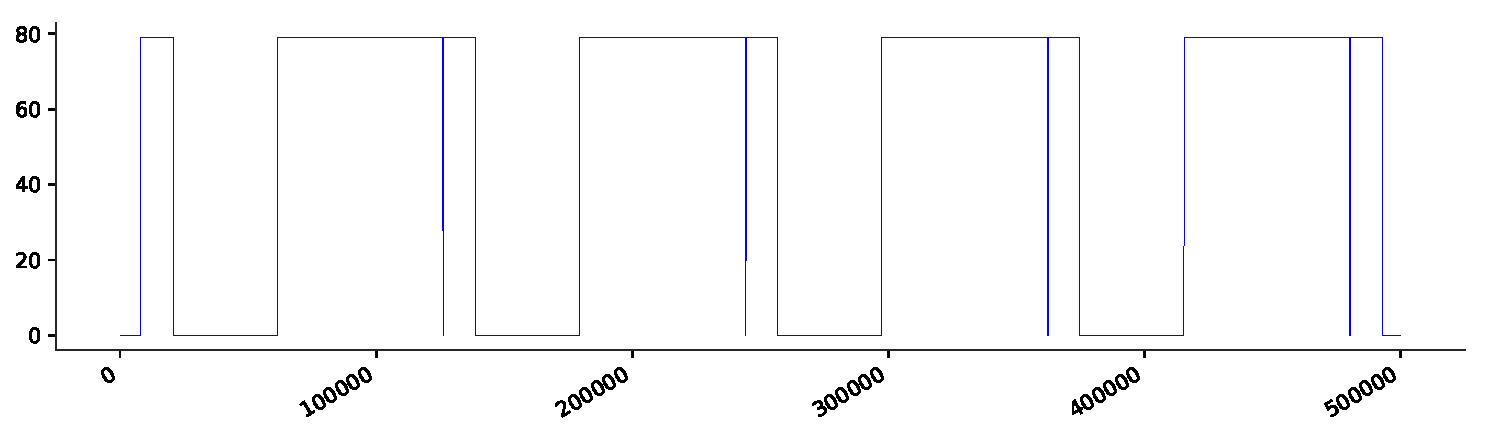
\includegraphics[scale=0.6]{traces/oper_trigger_trace}
	\captionof{figure}{Power trace that indicates at which samples the doubling and addition operations start and end. Instead of taking the whole doubling operation into account, we only determine where the very first squaring happens. This explains why the doubling operation consist of less samples than the addition operation. }
	\label{fig: oper_trigger_trace}
\end{figure}
%
Given this power trace, we need to determine the indices at which a rising edge starts and how long it stays high (i.e. determine the relative index of the start of the corresponding falling edge).
Initially, our approach was to calculate the difference between consecutive elements in this trigger trace without any preprocessing. 
If the difference of two successive elements is high, it indicates that we are approaching a rising/falling edge (depending on the sign of this difference).
The success of this approach however depends on the sampling rate used.
If a low sampling rate is used, the difference between two successive elements can be higher.
In the case of a higher sampling rate, this difference will be much smaller.
Therefore, it is hard to choose a correct threshold to determine the indices of the rising and falling edges in this trigger trace.
To solve this, we decided to preprocess the trace by rounding all values below a threshold to zero.
One has to make sure that this threshold is lower than the values between a rising and falling edge.
Applying the method we described first now correctly yields the offsets at which operations start and end.

The previously described method still depends on the vertical offset of the operation trigger trace. 
A method that works regardless the vertical offset is shown in \Cref{algo: determining offsets}.
In the end, we decided to stick with this generic method.
The algorithm works by first determining the average of the minimum and maximum value in the trigger trace.
We then determine the greatest lower bound (GLB) and least upper bound (LUB) for all values smaller and bigger than this average respectively.
Our threshold $\mu$ now becomes the average of GLB and LUB.
All values in the trigger trace that are bigger or equal to this threshold are clipped to the maximum value, while values smaller are clipped to the minimum value. 
We then calculate the consecutive differences of all the samples in this trigger trace.
We can now determine the rising and falling edge indices by checking whether these absolute differences are bigger than our threshold $\mu$.
The offsets can now easily be found by taking the difference between these indices.
Given a pair of successive edge indices, only those indices are taken into account for which the first edge index corresponds to a rising edge (i.e. has a positive difference or its value is bigger than $\mu$).
%
\begin{algorithm}
	\algorithmicrequire A power trace $T$ of the trigger that indicates when one or more doubling/addition operations start/end. \\
	\algorithmicensure The offsets and durations to these operations.
	%	
	\begin{algorithmic}[1]
		\State $\text{min\_max\_avg} = (\max(T) + \min(T)) / 2$
		\State $T_H = \{s \mid s \in T, s \ge \text{min\_max\_avg} \}$
		\State $T_L = \{s \mid s \in T, s < \text{min\_max\_avg} \}$
		\State $\text{lub} = \sup(T_H)$ \Comment{Least Upper Bound (LUB)}
		\State $\text{glb} = \inf(T_L)$ \Comment{Greatest Lower Bound (GLB)}
		\State $\mu = (\text{glb} + \text{lub}) / 2$
		\State For all $s$ in $T$: if $s \ge \mu$ clip value to $\max(T)$, else clip value to $\min(T)$
		\State $\texttt{succ\_diffs}= \{T[n + 1] - T[n] \mid n \in [1, \#T) \}$ \Comment{Calculate the first order difference}
		\State $\texttt{edges} = \{\operatorname{idx}(d) + 1, d\in D \mid \abs{d} \ge \mu \}$ \Comment{Determine offsets}
		\State $\texttt{offsets} = \{(\texttt{edges}[n], \texttt{edges}[n + 1] - \texttt{edges}[n]) \mid n \in [0, \#\texttt{edges} ], \texttt{offsets}[n] > \mu \}$
		\State \textbf{Return} $\texttt{offsets}$
	\end{algorithmic}
	%
	\captionof{algorithm}{Given a power trace that contains the signals of the operations to attack, determine the offsets to these operations.}
	\label{algo: determining offsets}
\end{algorithm}
%